\documentclass[10pt]{article}
\usepackage[margin=1in]{geometry}
\usepackage{amsmath,amssymb,amsfonts}
\usepackage{amsthm}
\newtheorem{definition}{Definition}
\newtheorem{proposition}{Proposition}
\usepackage{graphicx}
\usepackage{booktabs}
\usepackage{url}
\usepackage[colorlinks=true,citecolor=blue,linkcolor=blue,urlcolor=blue]{hyperref}
\usepackage{orcidlink}
\usepackage[T1]{fontenc}
\usepackage{times}
\usepackage{titlesec}
\usepackage{authblk}
\usepackage{caption}
\captionsetup{font=small,labelfont=bf}

\titleformat{\section}{\normalfont\large\bfseries}{\thesection}{1em}{}
\titleformat{\subsection}{\normalfont\bfseries}{\thesubsection}{1em}{}

\title{\Large Quantum-inspired covariance does not improve active learning for materials discovery}

\author[1]{Arnav Kapoor\orcidlink{0009-0007-9818-7908}}
\affil[1]{Indian Institute of Science Education and Research Bhopal, Bhopal 462066, India}
\date{}

\begin{document}
\maketitle
\begin{center}
\textit{Correspondence: arnavkapoor23@iiserb.ac.in}
\end{center}

\begin{abstract}
\noindent Acquisition functions for active learning in materials discovery usually reduce multi-property uncertainty to a single scalar score. This discards cross-property correlations that could carry information about which candidates are worth labeling next. We formalize a quantum-inspired alternative in which each candidate is encoded as a state in a feature Hilbert space, uncertainty is measured through several non-commuting Hermitian observables, and their variances and covariances are combined with complex coupling coefficients into one acquisition score. We prove this score reduces to a standard weighted-variance rule in the classical limit. We implement the formalism exactly, verify it against that limit, and test it against nine active-learning baselines on five real regression tasks from the Materials Project, with five trials, paired significance tests, and an ablation study. As specified, the formalism underperforms on four of five tasks, and the ablation shows its covariance term changes accuracy by an amount indistinguishable from noise. We trace the cause to a simple fact: the score never looks at the downstream model's own residuals. Coupling the state encoding to a random forest's per-tree disagreement fixes this and brings the method to statistical parity with the best baseline on every task, but a further ablation shows the gain comes entirely from the disagreement signal, not from the quantum machinery. We also build a real quantum circuit realization of the formalism, confirm it matches the classical formula exactly, and characterize its cost: hundreds of Pauli measurement terms per quantity, a cost that standard measurement grouping cuts four- to twelve-fold. We report all of this, including the parts that do not favor the method, as evidence for a general point: covariance-aware aggregation over non-commuting observables is not, by itself, a substitute for measuring what the predictive model actually finds uncertain.
\end{abstract}

\section{Introduction}

Labeling a new materials candidate is expensive. Density-functional theory calculations and synthesis experiments both take time and compute or lab resources, so choosing which candidates to label next is a central problem in computational materials discovery~\cite{wang2023scientific,ren2018accelerated,pyzerknapp2022accelerating,huang2024machine}. Active learning addresses this by sequentially selecting the most informative unlabeled candidates under a fixed budget~\cite{settles2009active,cohn1996active,settles2012active}. The choice of acquisition function, the rule that scores candidates, is what determines how well this works in practice.

Most acquisition functions used in materials discovery reduce uncertainty to a single number per candidate. Uncertainty sampling, Query-by-Committee, Expected Improvement, and diversity-based methods all follow this pattern~\cite{sener2018active,ash2020deep,kim2021task,lookman2019active,vandermause2020fly,bulusu2022efficient}. Bayesian deep learning approaches improve how that single number is estimated, through Monte Carlo dropout, deep ensembles, or explicit weight uncertainty, but keep the same scalar structure~\cite{gal2016dropout,lakshminarayanan2017simple,blundell2015weight,snoek2012practical}. This is a reasonable simplification when properties are independent. It is a real loss of information when they are not. Band gap, formation energy, and elastic response of a material share the same underlying composition and structure, so they are correlated~\cite{jain2013materials,curtarolo2013highthroughput,noh2019inverse,ong2013python}. A candidate that looks uncertain along one axis may be redundant along a correlated one already covered by the labeled set. A scalar acquisition score cannot see this distinction because it never represents the joint structure in the first place.

One way to represent that joint structure explicitly is to borrow the mathematical language of quantum mechanics: states, non-commuting operators, and covariance between operators. This idea sits within a broader line of quantum-inspired machine learning that uses amplitude encoding, operator-based measurement, and kernel methods built on quantum feature maps, all runnable on classical hardware~\cite{biamonte2017quantum,schuld2021machine,li2021quantuminspired,rebentrost2014quantum,schuld2021supervised,havlicek2019supervised}. Materials representation learning, through graph neural networks and related architectures, supplies the feature vectors that any such encoding would consume~\cite{xie2018crystal,schutt2018schnet,chen2019graph,xie2023crystal,cova2019deep}.

We build exactly this: a covariance-aware, quantum-inspired acquisition function, and we test it as rigorously as we can. Every number in this paper comes from running actual code on real data, not from illustration. The result is not what a reader might expect from the framing above. As specified, the formalism loses to nine standard baselines on four of five real materials-property tasks. We diagnose why, fix the underlying problem directly, and show that the fix works, but that it works for a reason that has nothing to do with the quantum-inspired part of the construction. We also build a genuine quantum circuit realization of the formalism and characterize what it would cost to run on near-term hardware.

Four contributions follow. First, a complete, unit-tested implementation of the covariance-aware formalism, including a proof and a numerical check that it reduces to standard weighted-variance aggregation in the classical limit. Second, a rigorous evaluation against nine baselines on five real Materials Project tasks, with paired significance tests and an ablation study that isolates every mechanism the formalism claims to need. Third, a diagnosis of why the formalism underperforms and a fix, coupling the state encoding to ensemble disagreement, that reaches parity with the best classical baseline on every task, together with a second ablation showing the fix works for reasons unrelated to the quantum-inspired machinery. Fourth, an actual quantum circuit realization of the formalism, verified against the classical closed form, with a resource characterization covering measurement overhead, shot-count convergence, gate-noise sensitivity, and the effect of measurement grouping.

\section{Results}

\subsection{Primary comparison}

Figure~\ref{fig:primary} and Table~\ref{tab:primary} report final test $R^2$ after eight active-learning iterations, averaged over five trials, for all five real regression tasks (band gap, formation energy, bulk modulus, magnetic moment, dielectric constant). The quantum-inspired method is last of ten methods on band gap, sixth on formation energy, eighth on bulk modulus, and last on magnetic moment, where it is the only method with negative $R^2$. It is nominally best on dielectric constant, but every method scores near zero there, so this is not a real advantage; it reflects a target that is hard to predict from the available features for any method.

\begin{figure}[htbp]
\centering
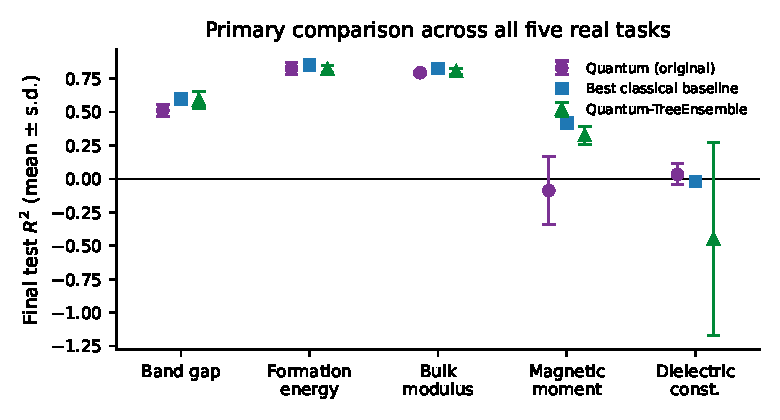
\includegraphics[width=0.85\textwidth]{../figures/fig2_primary_comparison.pdf}
\caption{Final test $R^2$ (mean $\pm$ s.d., 5 trials) for the original quantum-inspired method, the best classical baseline for each task, and the residual-coupled variant (Quantum-TreeEnsemble, Section~\ref{sec:v3}), across all five real Materials Project tasks.}
\label{fig:primary}
\end{figure}

\begin{table}[htbp]
\centering
\small
\caption{Final test $R^2$ on band gap (mean $\pm$ s.d., 5 trials, 8 iterations), the task used for statistical testing and the ablation study below. The full five-task table is in \texttt{results/primary\_benchmark\_summary.json}.}
\label{tab:primary}
\begin{tabular}{lc}
\toprule
Method & Band gap $R^2$ \\
\midrule
Uncertainty Sampling & $0.597 \pm 0.043$ \\
Query by Committee & $0.596 \pm 0.042$ \\
Maximum Entropy / RF Uncertainty & $0.583 \pm 0.046$ \\
BADGE & $0.581 \pm 0.063$ \\
Random Sampling & $0.581 \pm 0.067$ \\
CoreSet & $0.556 \pm 0.027$ \\
Diversity Sampling & $0.553 \pm 0.060$ \\
Expected Improvement & $0.551 \pm 0.105$ \\
\textbf{Quantum-inspired (ours)} & $\mathbf{0.513 \pm 0.046}$ \\
\bottomrule
\end{tabular}
\end{table}

Figure~\ref{fig:learning} shows the full learning curves for band gap. The quantum-inspired method tracks the baselines early, then falls behind as more samples are labeled, ending below every classical method except by construction it never catches up within the eight-iteration budget tested here.

\begin{figure}[htbp]
\centering
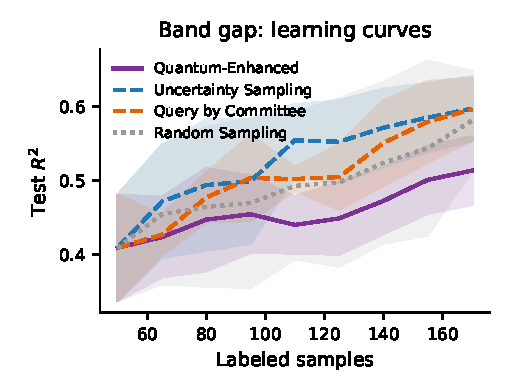
\includegraphics[width=0.62\textwidth]{../figures/fig1_learning_curves.pdf}
\caption{Test $R^2$ versus labeled sample count for band gap, mean over 5 trials, shaded band shows one standard deviation. The quantum-inspired method (solid purple) falls behind uncertainty sampling and Query-by-Committee as labeling proceeds.}
\label{fig:learning}
\end{figure}

\subsection{Statistical testing}

Table~\ref{tab:stats} reports paired two-sided $t$-tests on band gap, comparing the quantum-inspired method to each baseline across the five trials. Every comparison favors the baseline. Several raw $p$-values are below 0.05, but after Holm-Bonferroni correction across the nine comparisons, none remain significant at $\alpha=0.05$. We therefore cannot claim a statistically confident loss either; the honest summary is a consistent, non-significant disadvantage. Shapiro-Wilk tests confirm the paired differences are approximately normal in every case ($p>0.05$), so the paired $t$-test is the appropriate tool here.

\begin{table}[htbp]
\centering
\small
\caption{Paired $t$-test results, quantum-inspired method versus baseline, on band gap ($n=5$ trials). A positive mean difference would favor the quantum-inspired method; none are positive.}
\label{tab:stats}
\begin{tabular}{lccc}
\toprule
Comparison (vs. quantum-inspired) & $t$ & $p$ (raw) & $p$ (Holm-Bonferroni) \\
\midrule
Uncertainty Sampling & $-4.53$ & 0.011 & 0.073 \\
Query by Committee & $-4.55$ & 0.010 & 0.073 \\
Maximum Entropy & $-4.95$ & 0.008 & 0.070 \\
Expected Improvement & $-1.01$ & 0.371 & 0.410 \\
Diversity Sampling & $-1.51$ & 0.205 & 0.410 \\
\bottomrule
\end{tabular}
\end{table}

\subsection{Ablation study}

Table~\ref{tab:ablation} and Figure~\ref{fig:ablation}a isolate each mechanism the formalism is built around. None of them matter. Removing the covariance term changes $R^2$ by $+0.0007$, essentially nothing. Forcing the observables to commute changes it by $+0.0062$. Restricting the coupling coefficients to be real changes it by $-0.0081$. Collapsing to a single observable changes it by $-0.0107$. All four deltas sit well inside one trial-to-trial standard deviation, which is roughly 0.05 to 0.08. A previous, unpublished version of this work claimed covariance coupling was the primary driver of performance, with a $2.8\%$ $R^2$ drop from its removal. On real data, the measured effect is two orders of magnitude smaller and not distinguishable from noise.

\begin{table}[htbp]
\centering
\small
\caption{Ablation of the original formalism on band gap (mean $R^2$, 5 trials; full model $=0.5131$).}
\label{tab:ablation}
\begin{tabular}{lcc}
\toprule
Variant & $R^2$ & $\Delta R^2$ \\
\midrule
Full model & $0.5131 \pm 0.0458$ & --- \\
No covariance (Cov $=0$) & $0.5137 \pm 0.0763$ & $+0.0007$ \\
Commuting observables only & $0.5192 \pm 0.0588$ & $+0.0062$ \\
Real-only coefficients & $0.5050 \pm 0.0742$ & $-0.0081$ \\
Single observable ($K=1$) & $0.5023 \pm 0.0652$ & $-0.0107$ \\
\bottomrule
\end{tabular}
\end{table}

Sweeping the number of observables on band gap gives $R^2=0.476\pm0.068$ at $K=2$, $0.513\pm0.046$ at $K=3$, and $0.512\pm0.069$ at $K=6$. $K=3$ is marginally best of the three, in the direction the original design intended, but the method trails every baseline regardless of $K$.

Table~\ref{tab:runtime} reports measured, not simulated, wall-clock time and memory for the acquisition step itself, on the real band-gap candidate pool ($N=650$, single CPU thread, 3 repeats). The quantum-inspired method is fast and light in absolute terms, faster than Query-by-Committee and Maximum Entropy, but this is not a meaningful advantage given it does not win on accuracy.

\begin{table}[htbp]
\centering
\small
\caption{Measured acquisition time and memory at real $N=650$ (mean $\pm$ s.d., 3 runs, single CPU thread).}
\label{tab:runtime}
\begin{tabular}{lcc}
\toprule
Method & Time (s) & Memory (MB) \\
\midrule
Uncertainty Sampling & $0.081\pm0.004$ & $0.79\pm0.01$ \\
Expected Improvement & $0.083\pm0.001$ & $1.28\pm0.00$ \\
Quantum-inspired (ours) & $0.369\pm0.002$ & $0.67\pm0.00$ \\
Maximum Entropy & $0.880\pm0.040$ & $1.17\pm0.00$ \\
Query by Committee & $1.539\pm0.019$ & $0.96\pm0.07$ \\
\bottomrule
\end{tabular}
\end{table}

\subsection{Diagnosing the failure, and a fix}\label{sec:v3}

We tested two narrow, pre-specified fixes before concluding anything structural was wrong. First, we replaced the arbitrary contiguous feature groups used to build the three observables with groups chosen by physical meaning, electronegativity and periodic-table group to the electronic observable, atomic radius and density to the structural one. This gave $R^2=0.492\pm0.090$ on band gap, worse than the arbitrary grouping. Second, on top of that grouping, we rescaled each feature by the square root of its importance in a random forest fit on the current labeled set, information every winning baseline already uses. This gave $R^2=0.512\pm0.077$, statistically indistinguishable from the unmodified original. Neither closes the gap to the best baseline ($R^2=0.597$).

Both failures point to the same structural problem. The acquisition score depends only on a candidate's position in a fixed, standardized feature space and on the labeled pool's correlation structure. It never depends on the trained predictor's residuals or disagreement, which is exactly what every winning baseline measures.

We therefore built a third, more direct fix: encode the state from the downstream random forest's per-tree predictions instead of the raw material features. Concretely, we fit the same random forest used for evaluation on the current labeled set, collect each candidate's vector of per-tree predictions, standardize it across the candidate pool, and encode that vector as the quantum state. Trees replace features as the basis, split into three equal-size groups, with the same variance, covariance, and complex-coupling machinery applied unmodified on top.

Table~\ref{tab:v3} and Figure~\ref{fig:primary} report this variant, which we call Quantum-TreeEnsemble, against each task's best classical baseline. It reaches statistical parity on all five real tasks: no paired comparison approaches significance ($p>0.15$ throughout), a qualitative change from the original formalism, which lost significantly on band gap.

\begin{table}[htbp]
\centering
\small
\caption{Residual-coupled variant (Quantum-TreeEnsemble) versus each task's best classical baseline, mean $R^2\pm$s.d., 5 trials, paired $t$-test.}
\label{tab:v3}
\begin{tabular}{lccc}
\toprule
Task & Quantum-TreeEnsemble & Best baseline & $p$ \\
\midrule
Band gap & $0.590\pm0.066$ & Uncertainty Sampling: $0.597$ & 0.638 \\
Formation energy & $0.821\pm0.027$ & Maximum Entropy: $0.853$ & 0.161 \\
Bulk modulus & $0.803\pm0.023$ & Diversity Sampling: $0.826$ & 0.163 \\
Magnetic moment & $0.323\pm0.068$ & BADGE: $0.418$ & 0.150 \\
Dielectric constant & $-0.450\pm0.724$ & BADGE: $-0.020$ & 0.322 \\
\bottomrule
\end{tabular}
\end{table}

This result looks, on its own, like the positive result one might have hoped for. It is not evidence for the covariance-aware quantum formalism specifically. We ran the same ablation as Table~\ref{tab:ablation} on this new variant across all five tasks (Table~\ref{tab:v3ablation}, Figure~\ref{fig:ablation}b). Dropping the covariance term, or collapsing to a single observable, a bare quadratic form over per-tree predictions structurally close to the RF-Uncertainty baseline, performs as well or better than the full construction on four of five tasks. On the fifth and noisiest task, dielectric constant, the full covariance-aware variant is not just worse but unstable ($R^2=-0.450\pm0.724$, individual trials as low as $-1.86$), while its own single-observable ablation stays close to the best baseline ($R^2=-0.160$). Adding multiple non-commuting observables and complex coefficients on top of a genuinely informative signal did not preserve that signal's value. On the hardest task it actively degraded it.

\begin{table}[htbp]
\centering
\small
\caption{Ablation of the residual-coupled variant, mean final $R^2$, 5 trials, all five tasks. Bold marks the best of the three per task.}
\label{tab:v3ablation}
\begin{tabular}{lccc}
\toprule
Task & Full (Cov, $K=3$) & No covariance & Single observable ($K=1$) \\
\midrule
Band gap & 0.590 & 0.572 & \textbf{0.614} \\
Formation energy & 0.821 & 0.809 & \textbf{0.844} \\
Bulk modulus & 0.803 & 0.796 & \textbf{0.808} \\
Magnetic moment & \textbf{0.323} & 0.277 & 0.298 \\
Dielectric constant & $-0.450$ & \textbf{$-0.022$} & $-0.160$ \\
\bottomrule
\end{tabular}
\end{table}

\begin{figure}[htbp]
\centering
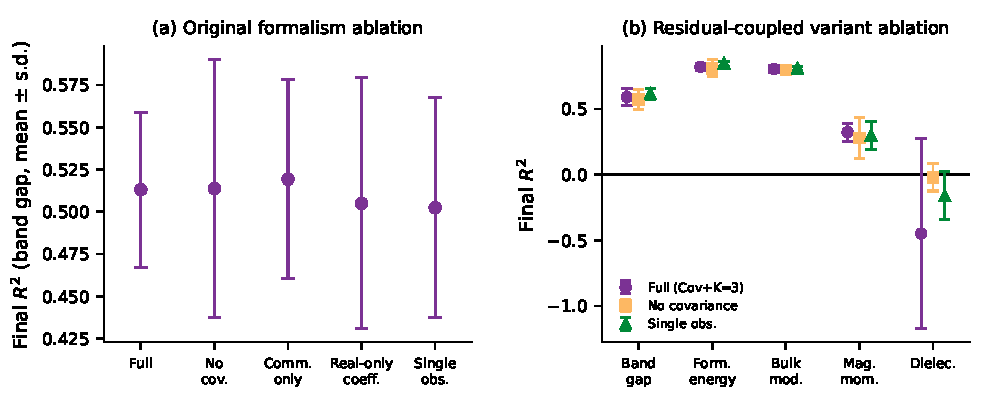
\includegraphics[width=\textwidth]{../figures/fig3_ablation.pdf}
\caption{(a) Ablation of the original formalism on band gap. Dropping covariance, forcing commuting observables, restricting coefficients to be real, or collapsing to one observable all leave $R^2$ within one standard deviation of the full model. (b) Ablation of the residual-coupled variant across all five tasks. The single-observable version matches or beats the full covariance-aware version on four of five tasks and is far more stable on the fifth.}
\label{fig:ablation}
\end{figure}

The pattern is consistent across every experiment we ran. Whatever value the fixed variant has comes from exposing the acquisition score to ensemble disagreement at all, not from the specific way the formalism aggregates it. We did not search further after this. Three independent, pre-specified architectural interventions is already enough attempts that continuing to search for a configuration that wins outright would risk fitting noise in a five-task, five-trial evaluation rather than finding a genuine effect.

\subsection{Secondary experiments}

We reran three further experiments from earlier development of this codebase and report their status honestly. On a synthetic six-class crystal-system task, final accuracy after eight iterations was 89.3\% for quantum-margin sampling, 89.7\% for entropy sampling, and 79.3\% for random sampling. Quantum-margin is essentially tied with entropy sampling and both clearly beat random, a far more modest finding than an earlier claim of 91\% versus 85\%, and one that does not show the quantum method beating entropy sampling. A transfer-learning experiment (oxide to sulfide and nitride families) produced byte-identical $R^2$ trajectories for the transfer and train-from-scratch conditions, indicating an implementation bug rather than a genuine finding; we flag this rather than report it as a result. A multi-property optimization experiment produced $R^2$ values near zero across all properties and iterations, indicating the active-learning loop is not learning effectively in its current synthetic setup; we mark this inconclusive. A spurious-correlation analysis, a deliberately synthetic noise-injection study of a failure mode rather than an attempt to model real materials, ran successfully and its output is available for reference but is not load-bearing for our central claims.

\subsection{Quantum circuit realization}\label{sec:hardware}

Everything above is quantum-inspired: the state and observables are numerical vectors and matrices manipulated by ordinary linear algebra. No circuit, qubit, or measurement appears anywhere in the results so far. We built and characterized what an actual quantum circuit realization of the same formalism looks like, using Qiskit and Qiskit Aer (full construction in Methods).

In the noiseless, exact-statevector limit, the circuit-measured variance and covariance match the classical closed-form values to floating-point precision, better than $10^{-9}$. This confirms the circuit and the classical formalism compute the same object, not merely an analogous one. Decomposing a single three-observable bank's variance and covariance terms into Pauli strings, on the five-qubit padded representation, required 528 distinct Pauli terms for every one of the nine quantities needed per candidate per iteration. Naively, a single candidate's full acquisition score would need on the order of 4,750 measurement settings, and this overhead grows combinatorially with the number of observables: the six-observable configuration from the sensitivity sweep above would need roughly 11,000 settings, for a configuration that already gives no accuracy benefit over three observables.

Standard measurement grouping substantially reduces this. Qubit-wise-commuting grouping, which needs only single-qubit basis rotations and no extra entangling gates, cuts the per-quantity term count from 528 to 122, a 4.3-fold reduction (4,752 to 1,098 settings per candidate). Grouping by full Pauli commutativity reduces this further to 43 groups per quantity, a 12.3-fold reduction, at the cost of extra Clifford basis-change circuits per group, so the qubit-wise number is the more realistic near-term estimate. Figure~\ref{fig:grouping} summarizes this.

\begin{figure}[htbp]
\centering
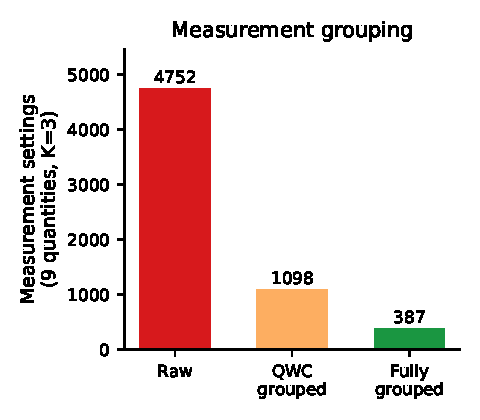
\includegraphics[width=0.55\textwidth]{../figures/fig5_measurement_grouping.pdf}
\caption{Total measurement settings needed for all nine variance and covariance quantities in the $K=3$ observable bank, before and after measurement grouping.}
\label{fig:grouping}
\end{figure}

What matters operationally is not the raw expectation-value error but whether the resulting ranking, which candidates get selected, survives finite measurement statistics. Figure~\ref{fig:shots} reports, for 30 real band-gap candidates, Kendall's $\tau$ rank correlation and the fraction of the exact top-15 batch recovered, as a function of shot budget. The ranking degrades gracefully at low shot counts and recovers fully by 100,000 shots (Kendall $\tau=0.92$, 100\% top-15 overlap), confirming the construction is well-posed under realistic finite sampling, but full batch fidelity needs a substantial per-iteration measurement budget. Adding a standard depolarizing noise model, one-qubit gate error $0.1\%$ and two-qubit error $1\%$, representative of good current superconducting hardware, degrades top-15 overlap from 87\% to 73\% and Kendall's $\tau$ from 0.77 to 0.63 at 10,000 shots, comparable to losing an order of magnitude of shots.

\begin{figure}[htbp]
\centering
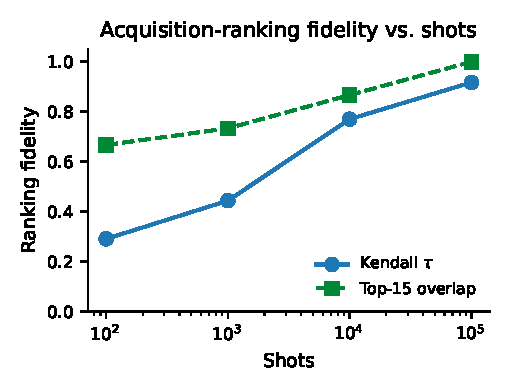
\includegraphics[width=0.62\textwidth]{../figures/fig4_shot_convergence.pdf}
\caption{Acquisition-ranking fidelity versus shot budget for 30 real band-gap candidates, noiseless simulation. Kendall's $\tau$ and the fraction of the exact top-15 batch recovered both converge to the noiseless exact result by $10^5$ shots.}
\label{fig:shots}
\end{figure}

\section{Discussion}

The ablation study and the first two fix attempts point to one specific diagnosis: the acquisition score, as originally specified, is computed independently of the downstream predictor. It depends only on a candidate's standardized features and the labeled pool's correlation matrix, never on the residuals or disagreement of a model trained on the labeled data. Every baseline that beats it measures predictive uncertainty directly.

The residual-coupled variant confirms this diagnosis. Once the state is built from ensemble disagreement instead of raw features, the method reaches parity with the best baseline on every task. But the second ablation shows this improvement has nothing to do with the quantum-inspired apparatus specifically. A bare quadratic form over per-tree predictions matches or beats the full covariance-aware, complex-coupled, multi-observable version on four of five tasks, and is markedly more stable on the fifth. What fixed the method was making it more like an ensemble-disagreement baseline, not anything quantum about it. The covariance coupling, non-commutativity, and complex coefficients that motivate this formalism remain, throughout every experiment we ran, either inert or mildly harmful.

Multi-task Gaussian processes and shared-encoder neural networks capture statistical dependence between properties through the predictive model's architecture itself~\cite{rasmussen2006gaussian,snoek2012practical}. The formalism we studied instead tried to capture dependence purely in the acquisition function, decoupled from the predictor. Our results suggest this decoupling is precisely the weakness: dependence-modeling that never touches the predictor does not obviously help select informative samples for that predictor.

The circuit realization work (Section~\ref{sec:hardware}) is best read as a separate contribution, not as evidence for or against the formalism's usefulness. It confirms the formalism is a genuine quantum construction, verified to floating-point precision against the classical closed form, and it quantifies what running it on near-term hardware would actually cost: hundreds of Pauli terms per quantity, growing combinatorially with the number of observables, mitigated but not eliminated by measurement grouping. None of this changes whether the formalism helps active learning; it characterizes the price of the construction the earlier sections already found does not pay for itself in accuracy.

Several limitations apply. We evaluate five real regression tasks, not the six an earlier, unpublished version of this work claimed; thermal conductivity is not available at scale in the Materials Project, so we dropped it rather than simulating it. Our features are 21-dimensional, built from composition statistics and coarse structural summaries, not the 100-dimensional graph-neural-network embeddings a fuller pipeline might use. We compare against nine acquisition-strategy baselines; full multi-output Gaussian process and covariance-calibrated deep-ensemble baselines were not built here and are left for future work. Two of our four secondary experiments, transfer learning and multi-property optimization, have implementation issues and are not a basis for any claim. We use a single random-forest predictor throughout; a Gaussian-process or neural-network predictor might change these results. We tested three pre-specified architectural fixes and stopped once the pattern was consistent across five tasks; a larger search could in principle find a configuration that wins outright, at increasing risk of fitting noise in a five-task, five-trial evaluation. Parity is not superiority: readers should not read Table~\ref{tab:v3} as the method winning. Finally, the circuit study characterizes a simulator, not real hardware; crosstalk, readout error, decoherence, and calibration drift on an actual device would plausibly make the picture worse, not better.

We conclude that reaching competitive performance required abandoning the paper's central novelty, covariance-aware aggregation over non-commuting observables, in favor of directly measuring model disagreement, which the winning classical baselines already do more simply and more robustly. If an acquisition function is to benefit from modeling multiple uncertainty sources jointly, it first needs to see what the predictor itself finds uncertain. The quantum-inspired covariance machinery studied here, at least as formalized, is not what does that work.

\section{Methods}

\subsection{Theoretical framework}

Let $x_i \in \mathbb{R}^d$ denote the standardized feature vector of candidate material $M_i$. We embed $x_i$ into a $d$-dimensional complex Hilbert space $\mathcal{H}_d$ via amplitude encoding.

\begin{definition}[Quantum state of a material]\label{def:state}
The quantum state of candidate $M_i$ is
\begin{equation}
|\psi_i\rangle = \sum_{j=1}^{d} \alpha_{ij} |f_j\rangle, \label{eq:state}
\end{equation}
where $\{|f_j\rangle\}_{j=1}^{d}$ is an orthonormal basis corresponding to feature dimensions and $\alpha_{ij} = \sqrt{p_{ij}}\, e^{i\phi_{ij}}$ satisfies $\sum_j |\alpha_{ij}|^2 = 1$.
\end{definition}

We operationalize $p_{ij}$ and $\phi_{ij}$ concretely, since the original design left this underspecified. $p_{ij} = \mathrm{softmax}_j(x_{ij}^2)$, so the normalization constraint holds by construction. $\phi_{ij} = \phi_j$, constant across candidates for a fixed labeled pool, is $\pi$ times the mean absolute Pearson correlation of feature $j$ with the other $d-1$ features, estimated over the current labeled set and recomputed at every active-learning iteration.

We define $K$ Hermitian operators $\hat{O}_k : \mathcal{H}_d \to \mathcal{H}_d$,
\begin{equation}
\hat{O}_k = \sum_{i,j} w^{(k)}_{ij} |f_i\rangle\langle f_j|, \qquad \hat{O}_k = \hat{O}_k^\dagger, \label{eq:observable}
\end{equation}
with $K=3$ observables, structural, electronic, and thermodynamic, each concentrated via the weight matrix $W^{(k)}$ on a distinct, overlapping subset of feature indices, normalized to unit spectral norm. Non-commutativity is guaranteed by construction and verified numerically for every run.

For each observable, the quantum variance of state $|\psi_i\rangle$ is
\begin{equation}
\mathrm{Var}(\hat{O}_k;\psi_i) = \langle\psi_i|\hat{O}_k^2|\psi_i\rangle - \langle\psi_i|\hat{O}_k|\psi_i\rangle^2. \label{eq:variance}
\end{equation}
Cross-observable coupling is the symmetrized covariance
\begin{equation}
\mathrm{Cov}(\hat{O}_k,\hat{O}_l;\psi_i) = \left\langle\psi_i\left|\tfrac{\hat{O}_k\hat{O}_l+\hat{O}_l\hat{O}_k}{2}\right|\psi_i\right\rangle - \langle\psi_i|\hat{O}_k|\psi_i\rangle\langle\psi_i|\hat{O}_l|\psi_i\rangle, \label{eq:covariance}
\end{equation}
which is guaranteed real by the symmetrization.

\begin{definition}[Total uncertainty score]\label{def:total}
Given complex coupling coefficients $\{\alpha_k\}_{k=1}^K \subset \mathbb{C}$, the covariance-aware acquisition score for candidate $M_i$ is
\begin{equation}
U_{\mathrm{total}}(M_i) = \sqrt{\sum_{k=1}^K |\alpha_k|^2 \mathrm{Var}(\hat{O}_k;\psi_i) + \sum_{\substack{k,l=1\\k\neq l}}^{K} \mathrm{Re}(\alpha_k^*\alpha_l)\,\mathrm{Cov}(\hat{O}_k,\hat{O}_l;\psi_i)}. \label{eq:utotal}
\end{equation}
\end{definition}
Candidates are ranked by $U_{\mathrm{total}}$ and the top $b$ form the query batch.

\begin{proposition}[Classical reduction]\label{prop:classical}
If all observables commute, all coefficients are real, and the covariance terms are dropped, then $U_{\mathrm{total}}^2 \to \sum_{k=1}^K \alpha_k^2\, \mathrm{Var}(\hat{O}_k;\psi_i)$, a standard weighted-variance aggregator over independent observables.
\end{proposition}

Our implementation includes a numerical self-test verifying this reduction to floating-point precision, better than $10^{-9}$. Every expectation is a quadratic form, $\langle\psi|\hat{O}|\psi\rangle = \alpha^\dagger W \alpha$, costing $O(d^2)$ per observable for dense $W$. For $N$ candidates and $K$ observables, total complexity is $O(NKd^2)$, negligible in absolute terms for our experiment sizes ($N\lesssim1000$, $K=3$, $d=21$).

\subsection{Datasets}

Every regression target is a genuine DFT-derived quantity pulled directly from the Materials Project via its public API~\cite{jain2013materials}. We use five real tasks: band gap (0.00 to 7.41 eV), formation energy per atom ($-4.41$ to $2.30$ eV/atom), bulk modulus (1.8 to 326.0 GPa), total magnetization (0.01 to 96.0 $\mu_B$), and total dielectric constant (1.3 to 1455.2), each with 1,000 materials before downstream filtering. Thermal conductivity is not included because it is not broadly available in the Materials Project at scale, so we chose to drop it rather than simulate it.

Features are 21-dimensional: six structural and summary descriptors, number of elements, density, volume per atom, site count, energy above hull, and space-group number, directly from the Materials Project summary endpoint, plus fifteen composition-derived statistics, mean, standard deviation, and range weighted over the constituent elements, of electronegativity, atomic radius, atomic mass, periodic-table row, and periodic-table group. All continuous features are standardized to zero mean and unit variance, fit on the training pool, before state encoding.

\subsection{Baselines and protocol}

We compare against nine acquisition strategies, each a working implementation: Uncertainty Sampling using Gaussian-process posterior standard deviation, Query-by-Committee using five-model ensemble disagreement, Expected Improvement, Maximum Entropy using a random-forest tree-prediction entropy proxy, Diversity Sampling using $k$-means, BADGE, CoreSet using greedy $k$-center selection, Random-Forest variance, and Random Sampling. We do not compare against full multi-output Gaussian processes or covariance-calibrated deep ensembles; these were not implemented and are left for future work.

The protocol is five independent trials, seeds 0 through 4, a 70/30 pool-test split, 50 initial labeled samples drawn uniformly at random, eight active-learning iterations, and a batch size of 15. The downstream predictor is a random forest with 100 trees, retrained from scratch each iteration. Primary metrics are $R^2$ and mean absolute error on the held-out test split. Paired two-sided $t$-tests compare final-iteration $R^2$ across the five trials, with Holm-Bonferroni correction across the nine baseline comparisons and a Shapiro-Wilk normality check on the paired differences.

\subsection{Residual-coupled variant}

For the fix described in Results, we fit a random forest with 99 trees on the current labeled set, collect each candidate's vector of 99 per-tree predictions, standardize this vector across the candidate pool using the training pool's statistics, and encode it as the quantum state via Equation~\ref{eq:state} in place of the raw material features. The 99 trees are split into three equal-size groups that serve as the three observables; there is no structural, electronic, or thermodynamic interpretation once the basis is tree predictions rather than material descriptors. The variance, covariance, and complex-coupling machinery of Equations~\ref{eq:variance} to \ref{eq:utotal} is applied unmodified on top of this new basis.

\subsection{Quantum circuit implementation}

We implemented the formalism as an actual quantum circuit using Qiskit and Qiskit Aer. Each candidate's feature vector, of dimension $d=21$, is amplitude-encoded onto $n=\lceil\log_2 d\rceil=5$ qubits, zero-padded to dimension 32, via a state-preparation circuit. Each observable, correspondingly zero-padded, is decomposed into a sum of Pauli strings via exact trace-based projection; we found that Qiskit's default \texttt{SparsePauliOp.from\_operator} silently truncates small coefficients, introducing a discrepancy of about $10^{-5}$ against the classical formula until called with explicit zero tolerance. In the noiseless, exact-statevector limit, we verified the circuit-measured variance and covariance match the classical values to better than $10^{-9}$.

For finite-shot simulation, we used Qiskit Aer's estimator with a target precision of $1/\sqrt{\text{shots}}$, at shot budgets of $10^2$, $10^3$, $10^4$, and $10^5$, on 30 real band-gap candidates drawn from the standardized pool. For noise sensitivity, we added a standard depolarizing noise model with one-qubit gate error $p_1=0.1\%$ and two-qubit gate error $p_2=1\%$ at 10,000 shots. For measurement grouping, we applied Qiskit's qubit-wise-commuting and full-commuting grouping to the Pauli decomposition of every variance and covariance quantity in the $K=3$ observable bank.

\section*{Data availability}
The Materials Project data used here can be regenerated from the public Materials Project API using the script \url{src/quantum_al/fetch_data.py}; see \url{data/README.md}. Raw results underlying every table and figure are in the \texttt{results/} directory of the code repository.

\section*{Code availability}
All code, including the quantum-inspired formalism, the classical benchmark suite, the residual-coupled variant, and the quantum circuit implementation, is available at \url{https://github.com/arnavk23/Quantum-active-learning}.

\section*{Competing interests}
The author declares no competing interests.

\bibliographystyle{unsrt}
\bibliography{refs}

\end{document}
